\chapter{Introduction}\label{ch:intro}

The \emph{IT-Security Awareness Penetration Testing Environment} (\ape)\cite{itsape} is a tool to analyse the awareness of a computer's user regarding IT-security. It measures the user's response to certain deployed \emph{artifacts} which differ from the user's familiar environment. Most of them are similar to real-world attack scenarios or share certain objectives with them.

There are multiple aspects to the user's response, one of them being the reaction speed. For measuring the user's reaction speed, one must determine the exact point in time from which on it is possible for him or her to interact with the artifact. As \ape~is a tool for the Microsoft Windows operating systems (which focus on a graphical user interface), a user is able interact with an artifact as soon as he or she can visually perceive it on the screen, or in Windows terms: on the \emph{desktop}.

The process of finding this point in time can not be done reliably by observing the currently running processes or even meta information about it. Only the visual information of the current desktop is useful in this case: An extra feature or tool was needed to perform an image detection algorithm on the current screen and decide whether the visual cues of the currently deployed artifact are present on the user's desktop.

The most important measure for this tool would be the \emph{sensitivity} of the classification, meaning the probability of successful detection of artifacts when they are actually present (\emph{true positives}). This term will be called \emph{detection rate} in the rest of this work. The counter-measure for this is the \emph{specificity} which describes the rate of \emph{true negatives}. A second, equally important measure is the resource consumption for execution, especially the execution time. As the detection rate is an obvious measure for such a tool, the execution time and resources are almost equally important to not disrupt the user's experience or distort the reaction analysis by \ape. The limitation on the resources is given by the environment that \ape~is mainly used in: low-tier office hardware.

The work at hand describes the design considerations and implementation details of such a tool, called \emph{\vad} (\emph{\vd}), and presents the results of an evaluation given the previously proposed measures. For this, chapter \ref{ch:rel-work} outlines some related publications and the differences to our approach. In chapter \ref{ch:methods}, the software design and technical details of the \vd~are explained. The evaluation setup and results can then be found in chapter \ref{ch:results}, followed by a conclusion in \ref{ch:conclusion}.

As \ape~is designed for computers running \emph{Windows 7} in the 32-bit version, the \vd~was built for this operating system specifically but can run on newer Windows versions as well. Written in C\#, it uses Microsoft's \emph{.NET framework} in version 4.7.2 \cite{dotnet4_7_2} and the \emph{OpenCV}-wrapper \emph{Emgu CV} in version 3.4.3 \cite{emgucv}.

\chapter{Related Work}\label{ch:rel-work}

In their paper about evaluation of UI patterns Bakaev et al. \cite{ref_web-uis} use image recognition functions to analyse the screenshot of a website and produce a machine-readable representation of it. This approach processes the screenshot in multiple steps: A black and white version of the screenshot is used for rectangle detection. Next, text sections are identified and recognized, before detecting special UI element types using a trained feature extractor. The results are then used to analyse composite structures and output a textual representation of the website.

While the task seems similar to the one presented in this report, the proposed analysis of screenshots has different goals and does not suit the requirements for the \vd: The full classification of the user's desktop screenshot before identifying possible candidates for artifacts would imply a high demand on resources and is not a necessary step. Since those candidates would then be compared to reference images of artifacts, one can skip the classification steps and use an image feature detector on the screenshots directly.

Aradhye et al. \cite{ref_spam-mails} present a way to classify image-based e-mails as spam using image analysis. Their approach features a way to analyse even for complex backgrounds and contents without using OCR: First, text regions are extracted by thresholding the intensity of the grayscale image several times and performing connectivity analysis on the outcomes. With these regions identified, they categorize the image based on features regarding text-density, color saturation and color heterogeneity. The features are then used to train \emph{Support Vector Machines} (\emph{SVMs}) to distinguish between different mail classes.

The key advantage of this way to classify images is that the spam images have distinct features to distinguish them from other images in mails. On one hand the \ape~artifact database is diverse and training SVMs for every artifact type would be a large task by itself. On the other hand it is not easy to distinguish the more advanced \ape~artifacts from \emph{normal applications} by a rigidly defined feature set. This is because the goal of most of the artifacts \ape~employs is an imitation of a usual application.

\footnote{Find a third related work.}

Since none of the related work matches the goals for the \vad, a new tool had to be implemented.

\chapter{Methods}\label{ch:methods}

This chapter begins with a description of the general software design, including a brief requirement analysis and the resulting decisions regarding the implementation. The second part introduces the technical backgrounds and algorithms used, and especially explains the choice and the details of the image recognition algorithms.

\section{Software Design}\label{sec:software-design}

The client of \ape~that gathers the user's reaction to the deployed artifacts runs on the user's PCs as a Windows service. Instead of implementing the \vad~as an additional feature of the \ape~service it is implemented as an external tool. This is to keep a modular approach in which software parts can easily be exchanged, and secondly to be able to give the individual processes an independent priority for execution, thus guaranteeing enough resources for the execution of the \ape~service.

The main reason the \vd~was designed to run on the same machines as the \ape~service instead of e.g. a server infrastructure with better hardware or other external hardware was the user's privacy:  As \ape~aims to collect the data anonymously or pseudonymously, transactions of highly sensitive data (such as screenshots of the current desktop) would contradict this goal.

The information on artifact types to detect are provided by a \emph{recipes repository} on the same computer containing reference images of the artifacts to be deployed. Furthermore, the \vd~only has to look for visual cues of a single artifact type per run, as the \ape~service will call it with information on the currently deployed artifact type.

\subsection{Requirement analysis}

To implement the \vd, the following main requirements were identified:

\begin{enumerate}
	\item \label{itm:req-detection} Robust and high detection rate for visual cues of artifact in screenshots of a Windows desktop.
	\item \label{itm:req-lowruntime} Low runtime of at most few seconds on low-tier office hardware.
\end{enumerate}

These requirements reflect the measures given for this task in the first chapter. The \ref{itm:req-detection} requirement mainly has influence on the choice of image recognition algorithms, while the \ref{itm:req-lowruntime} contradicts the use of a very resource-heavy algorithm (which would provide better results, generally speaking) and has influence on the parameters of the used algorithm. This could lead to a trade-off between the \ref{itm:req-detection} and the \ref{itm:req-lowruntime} requirement which is referred to in section \ref{sec:tech-bg}.

The visual cues of artifacts are -- in the use cases up to now\footnote{phrasing} -- those of Windows GUI objects.

Further analysis of the nature of \ape~and refinement of the main requirements lead to the following secondary requirements:

\begin{enumerate}\setcounter{enumi}{2}
	\item \label{itm:req-nocuda} No usage of parallel computing on the graphics card (e.g. with the CUDA Toolkit\cite{cuda}), CPU only.
	\item \label{itm:req-win7console} Windows 7 console program (32-bit).
\end{enumerate}

The \ref{itm:req-nocuda} requirement is a specification of the \ref{itm:req-lowruntime}, as low-tier office computers usually don't include a CUDA-enabled graphics card or a non-integrated graphics card at all. This requirement results in better versatility of the tool, but comes at cost of a higher runtime.

Given the deployment area for \ape~in the present and near future, the \ref{itm:req-win7console} requirement is due to the environment \ape~is mainly run in.

Finally, while easy maintainability of the source code is certainly desirable for all projects, it should be an extra focus of this project, as further development is most probably not done by the original author.

\subsection{Implementation decisions}

It was initially decided to use an existing library for image recognition rather than to implement the needed algorithms anew. The choice for an image recognition library fell to OpenCV, as it is licensed as \emph{Open Source} under the BSD license and arguably the most maintained and popular of such libraries with almost 20 million downloads \cite{opencv_downloads}. Other libraries for similar tasks exist, but they either focus more on machine learning like \emph{Google's Tensorflow} \cite{tensorflow}, are web-based APIs (mostly non-free) like \emph{Google's Vision API} \cite{vision_api} or \emph{Amazon Rekognition} \cite{rekognition}, or are not well maintained, such as \emph{VLFeat} \cite{vlfeat}.

Because the runtime performance is so important for this tool, it was not suitable to implement the program using an interpreted programming language. The usage of OpenCV limits the available compiled languages to C, C++ or Java, and using the wrapper Emgu CV also allows to use C\#.

The advantage of C\# is the possibility to use Microsoft's \emph{.NET Framework} \cite{dotnet4_7_2}. It allows to write efficient source code while having a vast collection of existing packages at one's disposal. The \emph{redistributable packages} of .NET 4.7.2 needed for executing .NET 4.7.2 programs are available per default on an (up-to-date) Windows 7 or later system. Furthermore, the speed differences between the execution of .NET's intermediate language in their \emph{Just-in-Time} compiler are nowadays insignificant to programs written in e.g. native C++. Therefore the \vd~is written in C\# and .NET 4.7.2, using OpenCV 3.4.3 via the Emgu CV wrapper.

In the first iteration of evaluation it was noticed that the used post-processing function by Emgu CV was faulty and it was decided to write an own implementation of it as a replacement (see subsection \ref{sec:tech-bg:subsec:outlier-rejection} for details).

\section{Technical backgrounds}\label{sec:tech-bg}

% Base process
The process of image recognition in the \vad~takes two input images per run, one model image and one observed image, and tries to recognize the model in the observed image. The model image is a reference image of the current artifact and the observed image is a screenshot provided to the program at execution time. Since the given artifact type may have multiple reference images for several characteristics, this process might be performed as many times as there are reference images, but exits as soon as a match between a reference and the screenshot was found. This is especially important for the performance, as the order of the artifact's reference images are directly affecting the runtime (see chapter \ref{ch:results}).

% 3 steps
The goal of the recognition process is to find a valid transformation matrix for the largest possible subset of the observed image's features to the model's features. If such a matrix can not be found for a subset of certain size, it is decided that no match exists. There are three major steps involved in the image recognition process: \emph{Feature detection and description}, \emph{feature matching} and \emph{outlier rejection}, while the last step includes finding a transformation matrix.

The first step yields a set of features extracted from the observed image. This is also done for all of the model images, but their feature set could be fetched from a cache if extracted in a previous run, which effects the performance (see chapter \ref{ch:results}). The features are represented as feature descriptors which are then matched with the model's descriptors, resulting in a set of candidates for features found in both images. These are then post-processed during outlier rejection to find a transformation matrix from one feature subset to the other while matching the most candidates. If there is such a matrix fitting to a certain percentage of the candidates (see subsection \ref{sec:tech-bg:subsec:outlier-rejection}) the \vd~will return the successful detection of the artifact (return value $0$). Otherwise, it will return that no match was found (return value $1$).

The last step can take advantage of the special visual properties of the deployed artifact's. There are three possibilities of transformation for Windows GUI objects: First, they can be translated versions of the artifact's reference images. In this case, the transformation matrix is easy to find. Secondly the GUI objects can be scaled in a sometimes complex manner, sometimes shifting sub-parts of the object to different locations and changing the aspect ratio between feature points. The combination of both transformation is the third possibility. It is hard to impossible to find a single transformation matrix for the last two transformations, but sometimes sub-parts of the image can be recognized more easily.

The following sections will describe the choice of algorithms for each step and their configuration details.

\subsection{Feature detection with ORB}\label{sec:tech-bg:subsec:feature-detection}

The set of available algorithms for feature detection were provided by the implementations in Emgu CV, respectively OpenCV. From those, as shown in secondary literature such as Tareen et al. \cite{orb_comparison}, ORB configured to find a limited amount of features provides the best combination of resource usage and result quality compared to the other three algorithms. This has been confirmed for the task at hand, but nevertheless the other feature detection algorithms that don't have copyright restrictions can be used for the first step via command line arguments.

% Orb explanation.
The ORB (\emph{Oriented FAST and Rotated BRIEF}) keypoint detector and descriptor is a ``very fast binary descriptor based on BRIEF [...], which is rotation invariant and resistant to noise'' \cite[p.~1]{orb}. It is specifically designed for real-time systems and low computing power, thus being faster than most of the other currently available methods \cite{orb, orb_comparison}. As the name states, it combines an enhanced version of the \emph{FAST}\cite{fast} keypoint detector with \emph{rotation-aware BRIEF}\cite{brief} descriptors, two fast and performance-saving techniques for themselves. \cite{orb, fast, brief}

The FAST (\emph{Features from Accelerated Segment Test}) detector \cite{fast} is a corner detector designed for real-time applications, working on pixel-regions with fixed radius. The ORB detector utilizes an extended version of the FAST detector with a patch radius of $9$. This radius has proven to yield the most reliable results, where reliability is defined as the rate of detecting the same corners in multiple views of an object. \cite{fast, orb}

The extended FAST detector employed in ORB is used to detect corners on a pyramid scheme for scale variants \cite{scale_pyramids} of the image. At instantiation of Emgu CV's implementation of ORB one can adjust the scale factor and number of levels for those pyramids. For the \vd~the preconfigured scale factor $1.2$ with $8$ levels was used. Since the \vd~currently responds poorly to scaled versions of the artifact's reference images these settings could be adjusted in future versions (see chapter \ref{ch:results}).

After detection, a \emph{Harris corner filter} \cite{harris_corner} for rejecting edges is applied to the top keypoints with the strongest FAST responses \cite{orb}. The feature finding and filtering process in the Emgu CV implementation of ORB is done until a configured amount of features are found (if possible), the preconfigured amount in Emgu CV being $500$ features. This was doubled for the \vd~to get up to $1000$ features per image, as a higher amount allows for better differentiation between the artifact types. For screenshots with pixel resolutions resembling those of low-tier office hardware and other common resolutions (see \cite{statctr}) an even higher amount of features affects the execution time negatively while not resulting in better matches.

There are more configuration parameters available for ORB, but the preconfigured values were found to be sufficient for the task.

\subsection{Descriptor matching}\label{sec:tech-bg:subsec:descriptor-matching}

The matching step tries to find one or more descriptor of the \emph{training set}, which are the descriptors of the model image, for each \emph{query descriptor}. Each descriptor of the observed image is used as a query descriptor. For feature matching, there are only two possibilities implemented in Emgu CV: Brute-force matching and \emph{FLANN} (\emph{Fast Library for Approximate Nearest Neighbor}) \cite{flann} based matching. There are different matching algorithms implemented for both of them, such as the \emph{k-nearest-neighbor} algorithm (\emph{k-NN}).

FLANN based \emph{k}-NN-matching performs best for large datasets with high dimensionality, but is less likely to find all possible candidates for matches. \cite{flann} The trade-off between speed and accuracy mentioned in section \ref{sec:software-design} lead to the use of FLANN based k-NN-matching to result in better runtime performance. For the \vd~$k$ was set to $2$, so that for each query descriptor, the $2$ nearest-neighbor descriptors from the training set are returned -- if possible. The choice of $k$ allows to apply several post-processing filters (see subsection \ref{sec:tech-bg:subsec:outlier-rejection}) to find a valid transformation matrix faster than without these filters.

\subsection{Outlier rejection}\label{sec:tech-bg:subsec:outlier-rejection}

The best matches for each query descriptor found in step two of the image recognition process are filtered in several steps before trying to find a transformation matrix using the \emph{Random Sample Consensus} (\emph{RANSAC}) \cite{ransac} algorithm. These filtering steps try to exclude as many match candidates as possible from the given set so that the program can abort early if there are not enough match candidates left. The match candidates that do not match the correct features are called \emph{outliers}, while the ones that do are called \emph{inliers}.

\begin{figure}[h!]
	\centering
	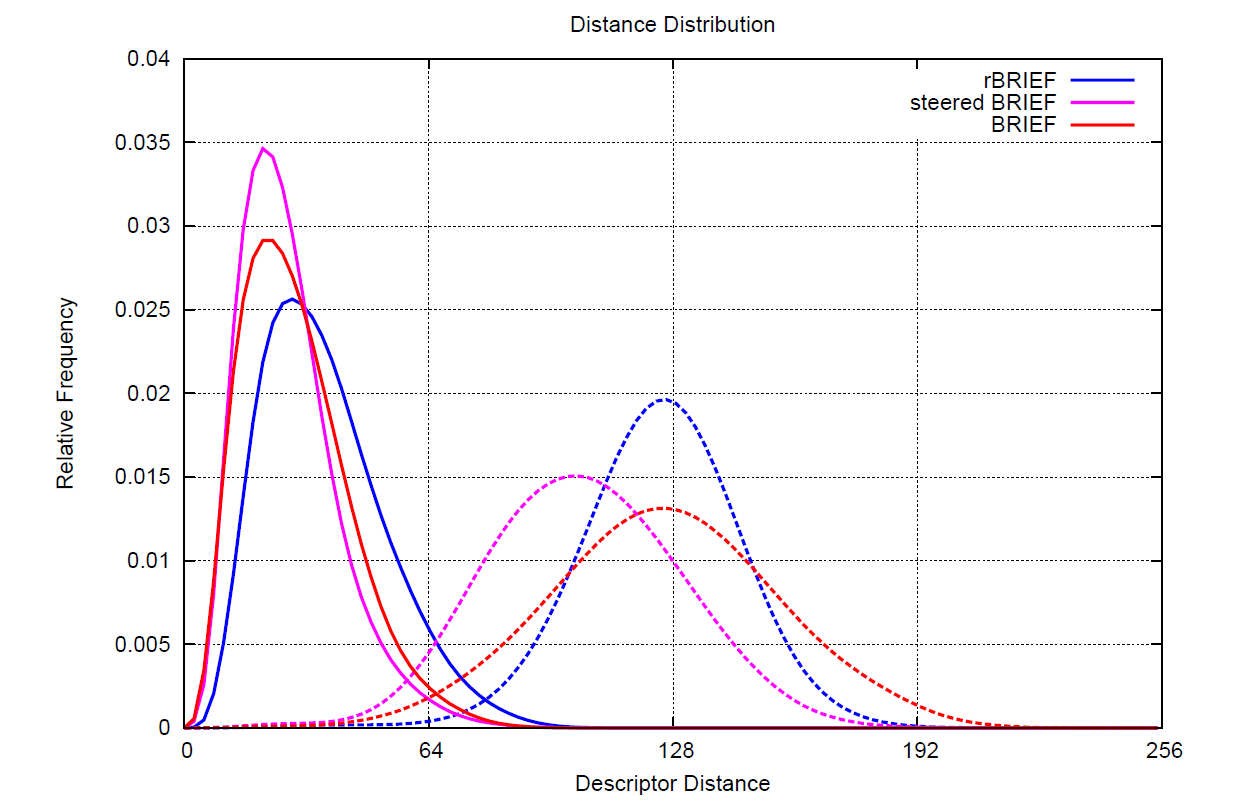
\includegraphics[scale=0.2]{fig/distance_threshold_orb.png}
	\caption{Analysis of the relation between descriptor distance and frequency, dotted for outliers and solid for inliers, taken from cite[p.~4]{orb}}\label{fig:dist-thresh}
\end{figure}

Since the 2-NN-matching can yield one match for query descriptors, only those descriptors that have two matches are taken into account for the next steps. The first test applied to each of the query descriptors' two matches is the distance threshold filter proposed in the original ORB publication \cite{orb}. Their analysis of the distance of a match compared to the probability of it being an inlier or outlier showed, that above a certain distance a match candidate is unlikely to be an inlier. For the \vd~a threshold of $80$ was chosen, as it is the approximate turning point of the probability for the candidate being an outlier rather than an inlier (see figure \ref{fig:dist-thresh}). The second filter is an implementation of \emph{Lowe's ratio test} \cite{lowes_ratio} with the recommended distance ratio of $0.7$ between the first and the second match's distance. After these steps, two functions provided by OpenCV/Emgu CV are used to eliminate duplicates and to rule out candidates that do not have the size and orientation of the majority of match candidates.

Between and after those filtering steps the \vd~determines the current count of match candidates and checks if there are still enough for a successful match. They are compared to a fixed parameter of $25$ divided by the ratio of the observed and model images' areas. This parameter of $25$ has been found empirically to be the best trade-off between a suitably high detection rate and early abortion of the matching process. The ratio of the image's areas allow model images to be found that have a small image size comparison to the observed image. This is a necessary factor, as the density of the feature descriptors per image area becomes more sparse if the image size is larger. \footnote{phrasing}

As the last step of image recognition, if there are enough candidates left, an own implementation of RANSAC is performed. Two match candidates are randomly sampled and are used to calculate translation and scaling factors for a hypothetical transformation matrix. This hypothesis is then tested on all match candidates allowing an error of an $11x11$ pixel patch.\footnote{phrasing} If a certain percentage of candidates, given by the confidence parameter, support it, a match was found.

The iteration count was set to $1000$ iterations, derived from the squared fixed parameter $25$ of minimally required match candidates adjusted upward to the next power of ten to allow for an error margin, respectively a high area ratio factor. This iteration count allows RANSAC in the best case to combine each match candidate with every other. The confidence was set to 85\% via empirical analysis, meaning that only 15\% of the remaining candidates may be outliers of the hypothetical matrix.

\chapter{Results}\label{ch:results}

The \emph{Artifact Detector} was evaluated in an environment that should closely resemble the real world application domain of \ape. In section \ref{sec:eval-env} the evaluation setup is explained in detail.

The \ref{itm:req-lowruntime} requirement resulted in the implementation of a \emph{cache} for already processed data of artifact images from previous runs. This leads to drastic runtime improvements in consecutive runs, as up to about 40\% of the runtime can be saved when reusing the previously calculated data. This is shown in section \ref{sec:eval-results}.

% first: qualitative?

\section{Evaluation setup}\label{sec:eval-env}

For the evaluation, Windows 7 was setup on a virtual machine using Oracle VM VirtualBox\cite{virtualbox}. This allowed an easy setup and quick configuration of the available hardware. All official Windows 7 updates were installed on this VM up to those available at 25.03.2019.

The virtual machine was run with 2GB of RAM available and one core of an Intel Core i5-6600K CPU (3,50 GHz) set to a 40\% execution cap, resulting in a single virtual CPU at a speed of 1.4 GHz. These hardware settings were thought to approximate low-tier office hardware sufficiently enough to allow conclusions for the real-world application domain of \ape.

After installing the \vd~in the virtual machine using the installer provided a Batch-script runs it using data supplied in shared folders by the host system.

\section{Evaluation results}\label{sec:eval-results}

There are two aspects for the evaluation, reflecting the measures given in chapter \ref{ch:intro}: First, a quantitative analysis of the execution resources is presented, also proving the efficiency and runtime advantage of the implemented cache. Then a qualitative analysis of the detection rate (sensitivity and specificity) follows.

\subsection{Execution resources}

Since the tests are run in a virtual machine, built-in tools for VirtualBox have been used for measuring the resource consumptions.

\begin{figure}
	\centering
	\subfigure[Execution time for loading the searched artifact's reference images.]{
		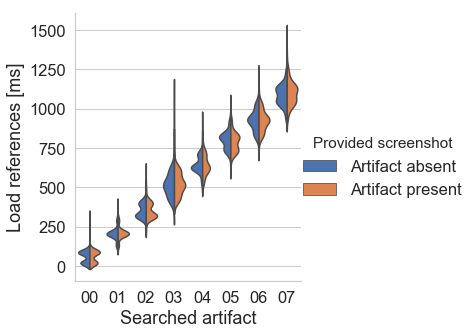
\includegraphics[scale=0.4]{fig/quantity-violin-load.png}\label{fig:result-quantity-load}
		}\qquad
	\subfigure[Execution time for extracting the observed screenshot's features.]{
		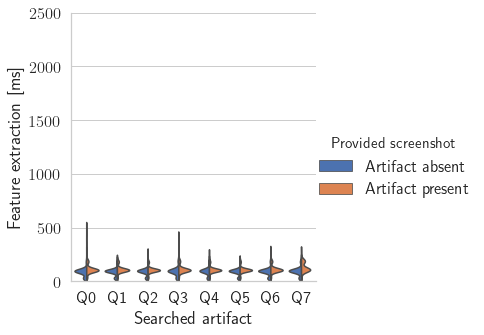
\includegraphics[scale=0.4]{fig/quantity-violin-feature_ext.png}\label{fig:result-quantity-feature_ext}
		}\\
	\subfigure[Execution time for matching the feature descriptors and finding a transformation matrix.]{
		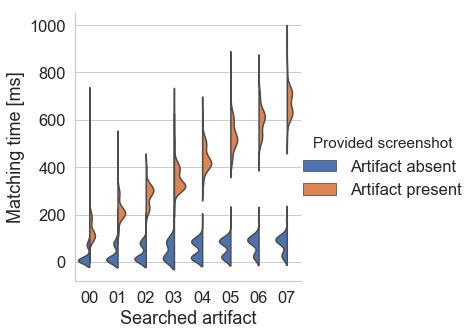
\includegraphics[scale=0.4]{fig/quantity-violin-matching.png}\label{fig:result-quantity-matching}
		}\qquad
	\subfigure[Execution time sum of all three image recognition parts.]{
		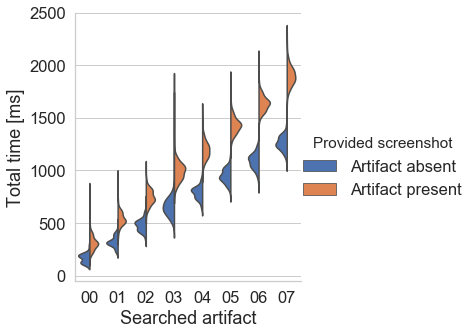
\includegraphics[scale=0.4]{fig/quantity-violin-total.png}\label{fig:result-quantity-total}
		}
	\caption{Measured execution times for artifacts 00 to 07}\label{fig:result-quantity}
\end{figure}

\subsection{Detection rate}

\begin{figure}
	\centering
	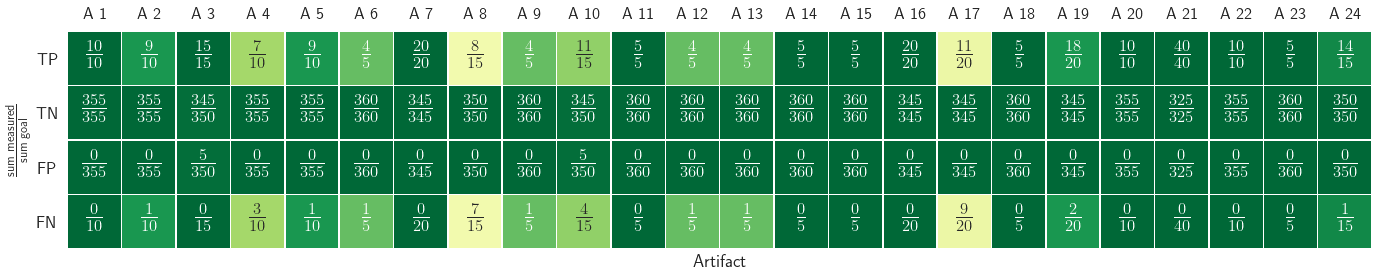
\includegraphics[scale=0.32]{fig/quality-confusion-matrix.png}
	\caption{Detection results for all runs by artifacts A 1 to A 24}\label{fig:result-quality-sum}
\end{figure}

\chapter{Conclusion}\label{ch:conclusion}

Possibly successful.
